\subsection*{Genome assembly of three medaka strains}
  Three medaka inbred strains were recently sequenced with PacBio single-molecule real-time (SMRT) sequencing and were assembled by the author's laboratory (Ichikawa \textit{et al}., unpublished; see Methods for an overview of the assembly procedure). Two strains (Hd-rR and HNI) were established from northern and southern Japanese populations, respectively and the other one (HSOK) was from eastern Korean population. The two Japanese populations are estimated to have separated 18 million years ago (MYA), whereas the ancestor of the two Japanese populations and that of the eastern Korean population are estimated to have separated 25 MYA \cite{Setiamarga2009}.


\subsection*{Genomic abundance of centromeric repeats}
  This study started with a candidate centromeric satellite sequence of medaka which was identified in a previous computational study \cite{Melters2013}. In that study, Melters \textit{et al.} estimated that the candidate centromeric satellite comprise 0.32\% of the medaka genome. However this estimation can underestimate the true genomic abundance due to its identification strategy. In order to better infer the genomic abundance of the centromeric satellite, PacBio raw reads were searched for the centromeric satellite sequence.

  Genomic fraction of the centromeric repeat was estimated by searching PacBio subreads for the representative monomer sequence with RepeatMasker \cite{Smit}. The genomic fraction in Hd-rR and HNI genomes were estimated to be $\sim$1\%, while that in the HSOK genome was $\sim$2\% (Table \ref{centromeric_repeat_genomic_abundance}). This difference is consistent with the previous observations that centromeric repeat array size in a chromosome can vary up to 20-fold among individuals within a species \cite{Miga2014}. Assuming the genome size to be 800 Mb, the centromeric satellite comprise 8--16 Mb of the genome, which implies each chromosome has around 500 kb of centromeric satellite on average. This is concordant with the observations that the centromere of many higher eukaryotes studied to date are characterized by hundreds to thousands of kilobases of satellite sequences \cite{Plohl2014}. Although quantifying the centromeric satellite in erroneous PacBio reads can lead to slight underestimation, the estimation should be more reliable than the clustering-based estimation using short Sanger reads in the previous study \cite{Melters2013}.


\subsection*{Centromeric repeat distribution}
  The distribution of the centromeric satellites in the three medaka genomes was investigated. The three assembled genomes were searched for the candidate centromeric satellite sequences using RepeatMasker (Table\,\ref{centromeric_repeat_distribution}, Fig.\,\ref{fig:repeat_distribution}). The results revealed that all the identified centromeric satellite arrays were truncated by contig gaps at either or both ends, suggesting none of the centromeric regions was spanned by a single contig. In the Hd-rR and HSOK genomes, $\sim$1-Mb centromeric satellites were identified in total, respectively, whereas only $\sim$80\,kb was identified in the HNI genome. This substantial difference in the amounts of identified centromeric satellite is presumably due to the difference in read length. The HSOK genome was sequenced with the newest P6-C4 chemistry and the average read length was 11\,kb; Hd-rR was sequenced with the combination of P6-C4 and older P5-C3 and P4-C2 chemistries and the average read length was 6.5\,kb; HNI was sequenced with P5-C3 and P4-C2 with the average read length of 3.6\,kb (Table\,\ref{sequencing_stats}). In addition, substantial amount of the centromeric satellite was identified in the contigs that failed to anchor to the chromosomes. The enrichment of identified centromeric satellite in unanchored contigs to in anchored contigs was as big as 12-fold in HSOK and 27-fold in HNI, in contrast to relatively small 3-fold enrichment in Hd-rR (Table\,\ref{centromeric_repeat_distribution}). In the Hd-rR genome assembly, contigs were scaffolded using BAC-/Fosmid-end sequencing reads and Hi-C contact frequency data, which successfully anchored a number of contigs containing centromeric satellites, emphasizing the effectiveness of complementing the long-read sequencing with other methods that capture even longer-range information.

  % TODO: describe that sum of satellites in the anchored and unanchored contigs did not reach the estimated abundance.

  For those chromosomes that have $>$1 kb centromeric repeat, positions of the centromeres in chromosomes were classified into metacentric, submetacentric, subtelocentric and acrocentric, employing the nomenclature by Levan \textit{et al.} \cite{levan1964} (Table\,\ref{centromeric_repeat_distribution}). Although this nomenclature originally based on karyotype observation rather than DNA sequence level and the positions induced from the two levels can slightly differ, the sequence-based classification conducted here is  nevertheless informative for interpreting subsequent analyses. The number of chromosomes classified to each type was in line with previous karyotype studies \cite{Uwa1981, Uwa1990}.

  Centromeric positions of the same chromosome were mostly conserved among the strains, confirmed by observing the corresponding pair of genetic markers flanked the repeat arrays, with only two exceptions in chromosomes 4 and 6 (Fig. \ref{fig:repeat_distribution}). For chromosome 4, Hd-rR had an acrocentric repeat array, whereas HSOK had a metacentric array. For chromosome 6, all the three strains had acrocentric repeat arrays but those of Hd-rR and HSOK and that of HNI located on the opposite end of the chromosome. As the karyotype study has revealed that the three strains possess slightly different sets of centromeric positions \cite{Uwa1990}, the difference of chromosomes 4 and 6 may be derived from \textit{bona fide} karyotype difference. Notably, Hd-rR chromosome 21 possessed metacentric and acrocentric arrays of nearly the same length (41.6 kb and 45.5 kb, respectively; Fig. \ref{fig:repeat_distribution}), thus this chromosome may dicentric where one of the arrays forms the functional centromere whereas the other is silenced.

  \begin{table*}[htp]
    \centering
    \caption{Centromeric repeat distribution}
    \begin{tabular}{r|rc|rc|rc}
  \hline
  & \multicolumn{2}{c|}{Hd-rR} & \multicolumn{2}{c|}{HNI} & \multicolumn{2}{c}{HSOK} \\ \hline
  chromosome & total repeat (bp) & position & total repeat (bp) & position & total repeat (bp) & position \\ \hline
  1  & 48,805  & SM  & 0      & -  & 0       & -  \\
  2  & 54,844  & M   & 3,831  & M  & 64,213  & M  \\
  3  & 52,681  & ST  & 0      & -  & 0       & -  \\
  4  & 10,513  & A   & 0      & -  & 305,521 & M  \\
  5  & 0       & -   & 10,605 & A  & 0       & -  \\
  6  & 8,226   & A   & 1,635  & A  & 7,020   & A  \\
  7  & 0       & -   & 12,911 & A  & 25,917  & A  \\
  8  & 59,863  & SM  & 0      & -  & 324,346 & SM \\
  9  & 40,159  & SM  & 0      & -  & 0       & -  \\
  10 & 0       & -   & 14,685 & ST & 0       & -  \\
  11 & 4,755   & A   & 4,513  & A  & 66,412  & A  \\
  12 & 232,280 & SM  & 25,683 & SM & 40,516  & SM \\
  13 & 35,778  & A   & 0      & -  & 0       & -  \\
  14 & 33,284  & A   & 0      & -  & 0       & -  \\
  15 & 0       & -   & 0      & -  & 63,112  & A  \\
  16 & 12,804  & A   & 0      & -  & 0       & -  \\
  17 & 1,588   & A   & 0      & -  & 0       & -  \\
  18 & 23,853  & SM  & 0      & -  & 9,236   & SM \\
  19 & 131,040 & SM  & 4,830  & SM & 4,757   & SM \\
  20 & 96,309  & ST  & 0      & -  & 17,574  & ST \\
  21 & 87,124  & M/A & 2,131  & A  & 0       & -  \\
  22 & 61,066  & A   & 0      & -  & 4,942   & A  \\
  23 & 6,580   & M   & 0      & -  & 25,847  & SM \\
  24 & 0       & -   & 0      & -  & 0       & -  \\
  \hline
  anchored total & 1,001,552 &  & 80,824 &  & 959,413 \\
  unanchored total & 3,279,256 & (5.89\%) & 2,254,882 & (3.16\%) & 11,273,168 & (17.5\%) \\
  total & 4,280,808 &  & 2,335,706 &  & 12,232,581 \\
  \hline
  positions summary & \multicolumn{2}{c|}{2M+6SM+2ST+8A (6U)} & \multicolumn{2}{c|}{1M+2SM+1ST+5A (15U)} & \multicolumn{2}{c}{2M+5SM+1ST+5A (11U)} &
  \hline
\end{tabular}

    \label{centromeric_repeat_distribution}
    \caption*{{\small
      Total amount of the centromeric repeats identified in the chromosomes are shown. The total amount in the contigs that were anchored to the chromosomes and in the unanchored contigs are also shown (fraction of the centromeric repeats in the unanchored contigs are shown in the brackets). The centromeric positions were determined by the repeat distribution on each chromosome, employing the nomenclature by Levan \textit{et al.} \cite{levan1964}. Hd-rR chromosome 21 possessed centromeric repeat arrays of nearly the same length (41.6 kb and 45.5 kb) at the positions corresponding to metacentric and acrocentric, thus described as 'M/A'. M, metacentric; SM, submetacentric; ST, subtelocentric; A, acrocentric; U, unknown (due to the lack of centromeric repeats).
    }}
  \end{table*}


\subsection*{Centromeric sequence mapping by FISH}
  To confirm that the candidate centromeric satellite sequence truly localizes to the centromeres, FISH experiment was conducted. Probe sequences were designed by the author and the FISH experiments were carried out by a collaborator (see Methods).

  The candidate satellite identified by Melters \textit{et al.} \cite{Melters2013} was first used as a hybridization probe and signals were observed only from 5$\sim$7 chromosome pairs (Fig.\,\ref{fish_each}). In order to map the centromeres of the other chromosomes, additional probes were designed (see Methods). The additional probes successfully hybridized to some chromosomes that the first probe failed to hybridize, with approximately the same positions as expected by the \textit{in silico} centromeric repeat distribution (Fig.\,\ref{fish_each}, Table\,\ref{centromeric_repeat_distribution}), although two additional probes hybridized to less chromosomes than expected by the \textit{in silico} alignment results. When all the probes combined, signals were observed at the centromeres of $\sim$13 pairs of chromosomes (Fig.\,\ref{fish_all}). This result confirmed that the candidate centromeric satellite truly derives from the centromeres. Moreover, the number of the chromosomes having each centromeric positions were largely consistent with the sequence-based results in the previous section.

  \begin{figure*}
    \centering
    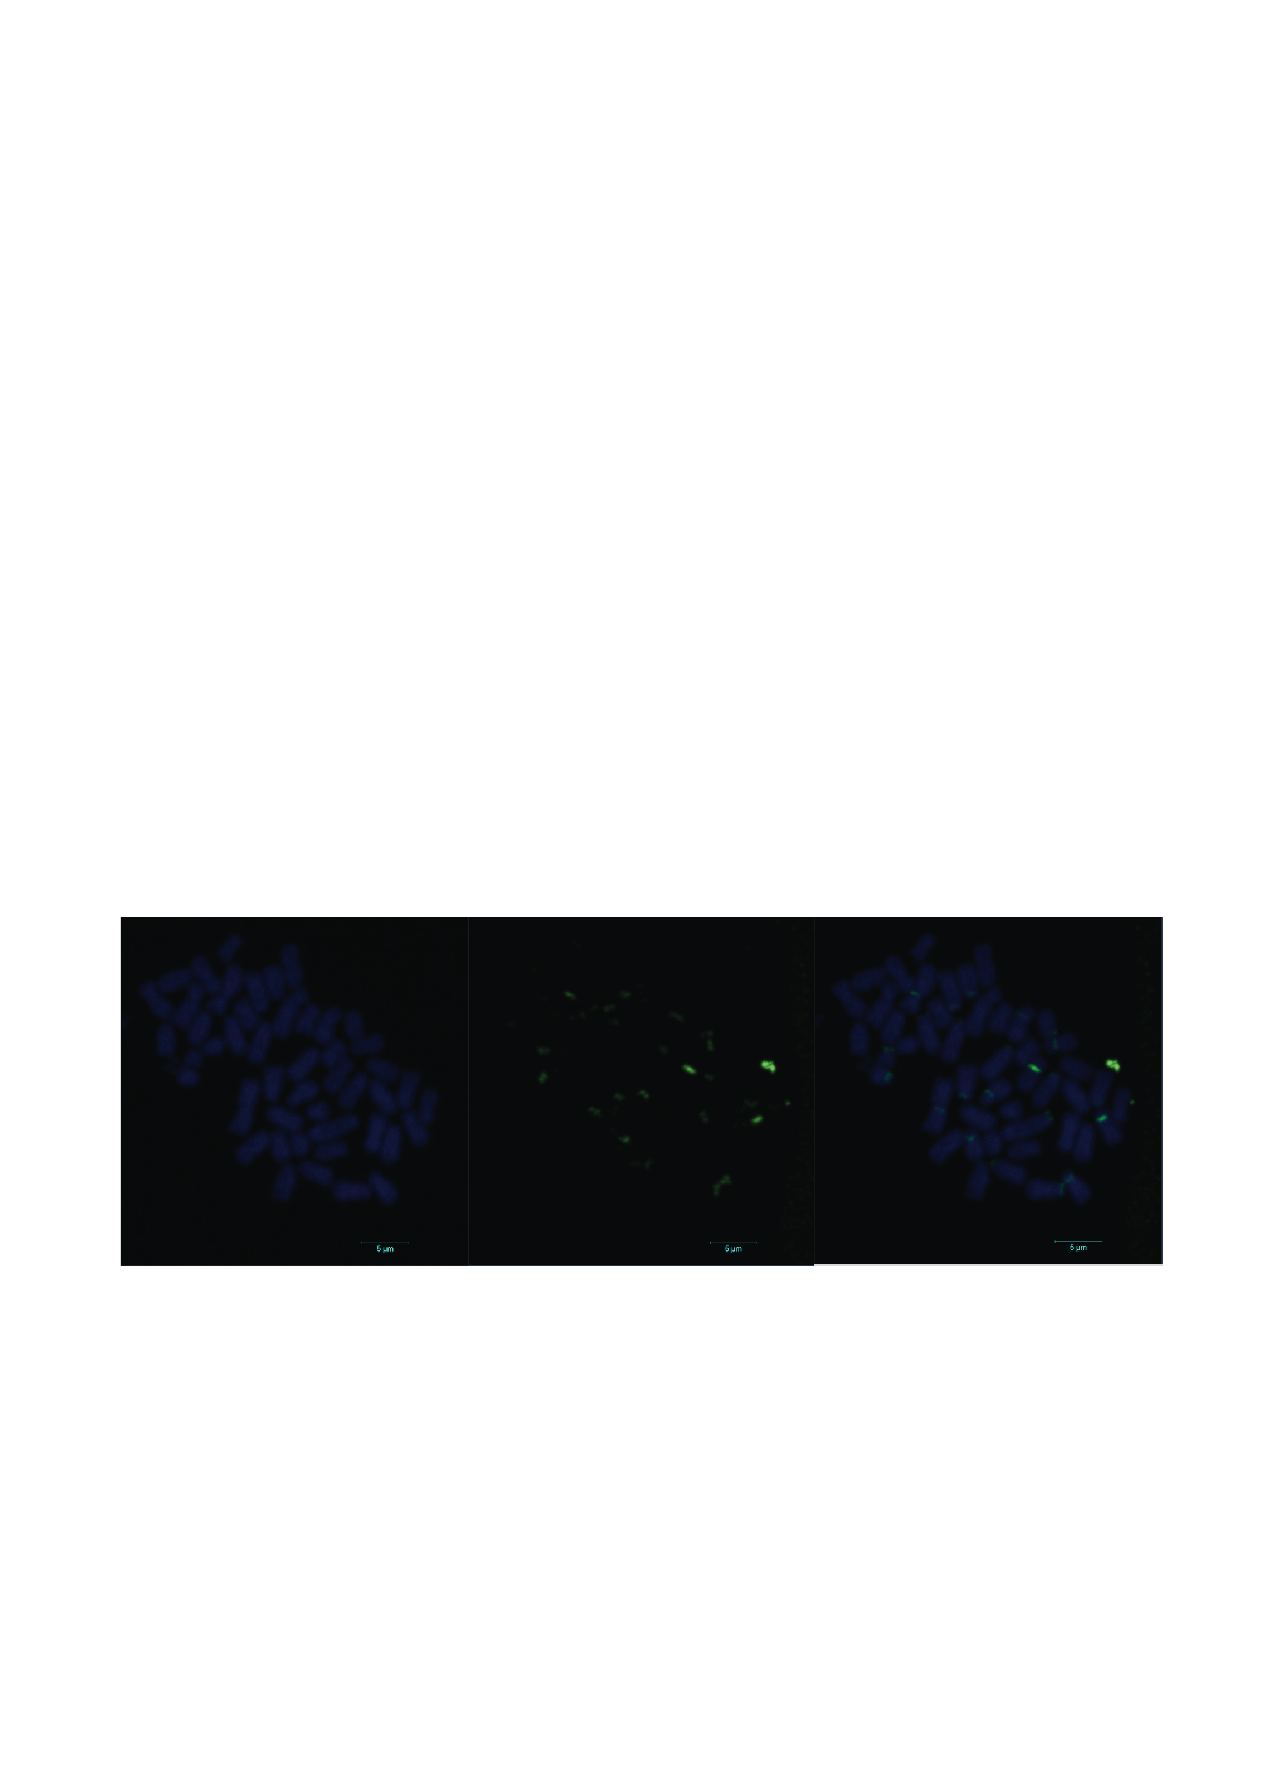
\includegraphics[width=\linewidth]{fish_all_probes.pdf}
    \caption{
      The candidate centromeric satellite sequence and three derivative sequences localized to the centromeres of $\sim$13 pairs of chromosomes. (left) DNA is stained with DAPI. (center) probes are stained green. (right) two images are combined.
    }
    \label{fish_all}
  \end{figure*}


\subsection*{Validation of centromeric sequence assembly}
  Repetitive nature of centromeric sequences inevitably accompanies the possibility of misassembly. In order to validate the centromeric sequence assembly, PacBio raw subreads were mapped to the assembled genomes and read coverage over centromeric regions was visualized for manual inspection.

  PacBio subread were mapped to the medaka genomes by BLASR \cite{Chaisson2012} with a stringent mapping parameters (see Methods). The assembly validity was then manually inspected on the genomic browser by confirming that enough number of subreads covered the centromeric repeat arrays without breaks. Most part of the centromeric sequences were covered by enough number of subreads, although a small number of exceptions were observed in chromosomes 9, 13 and 20 in the Hd-rR genome, which contained one or two breaking points that were not spanned by subreads (Fig.\,\ref{centromere_landscape}). Although PacBio read-based assembly validation cannot completely exclude the possibility of misassembly, indeed long-range ordering over the centromeric repeat arrays can be inaccurate, nevertheless relatively narrow range of assembly can be ascertained and that is adequately informative for observing sequence composition of a specific chromosome or inter-chromosomal sequence similarity.


\subsection*{Inter-chromosomal centromeric sequence conservation}
  It is widely known that in some species centromeric sequences exhibit inter-chromosomal conservation that are considered to derive from evolutionary rearrangements of chromosomes and/or frequent sequence exchange as a result of co-localization in the nucleus \cite{Willard1991}. In order to reveal the presence of inter-chromosomal relationship of centromeric repeats in the medaka genomes, satellite sequences from each chromosome were compared.

  Centromeric repeat arrays in each chromosome were decomposed into satellite monomers by RepeatMasker and the monomers were clustered by DNACLUST \cite{Ghodsi2011} with $>$85\% sequence similarity threshold. For those clusters that have $\geq$10 members, the monomer with the longest sequence in the cluster was chosen as the representative monomer of the cluster. All-vs-all pairwise alignment of the representative monomers from each chromosome along with the representative monomer identified by Melters \textit{et al}. was performed and pairwise distance was calculated. Based on this distance, hierarchical clustering of the chromosome-representative monomers were performed. The chromosome-representative monomers were clustered into four groups, revealing the presence of super-chromosomal subfamilies (Fig.\,\ref{monomer_clustering}, Table\,\ref{super_chromosomal_subfamily}). Many (15 out of 24) chromosomes (chr.\,2, 3, 5, 6, 7, 10, 11, 12, 14, 15, 16, 18, 20, 22 and 23) were assigned exclusively to one of the four subfamilies. Five chromosomes (chr.\,1, 4, 8, 13 and 19) were clustered into two or three subfamilies but significantly more monomers were classified to one subfamily over the others, thus they are assigned to the dominant subfamily. Chromosomes 9 and 21 were classified into two subfamilies with no significant preference. Chromosomes 17 and 24 could not be classified due to the lack or insufficient amount of centromeric repeats in either of the three assembled genomes. Overall, 22 out of 24 chromosomes were assigned to one or two subfamilies.

  Intriguingly, each subfamily exhibited distinct preference of centromeric positions in chromosomes; namely subfamily (SF) 2 for acrocentric, SF 1 and 3 for submetacentric and subtelocentric and SF 4 for metacentric, respectively (Table \ref{super_chromosomal_subfamily}). This tendency is analogous to the traditional observation that human acrocentric chromosomes share highly identical alpha-satellite sequences \cite{Willard1991}.

  In those chromosomes that had sufficient amount of centromeric repeats in multiple strains, most (7 out of 9) chromosomes were classified into the same subfamilies among strains. One of the exceptions was chromosome 19, where representative monomers from Hd-rR and HSOK were classified into SF 1 while that of HNI into SF 3, although the repeats from each strain were confirmed to locate in close position of the chromosome as they were flanked by a corresponding pair of genetic markers (Fig.\,\ref{fig:repeat_distribution}). This discordant classification may be because the assemblies of each strain captured different subregion of the corresponding repeat arrays or due to misassembly in one or more strains. The other exception was chromosome 21, where the representative monomers from the acrocentric array of Hd-rR were classified into SF 2, those from the metacentric array of Hd-rR and from the acrocentric array of HNI into SF 3. The two acrocentric arrays from Hd-rR and HNI were located at close but distinct positions in the chromosome (Fig.\,\ref{fig:repeat_distribution}), thus it may well contain different repeat sequence profiles and be classified into different subfamilies. The overall conservation of centromeric satellites among the three strains which separated 18 and 25 million years ago is in line with the previous observation that centromeric sequences were conserved among species within about 50 million years after separation \cite{Melters2013}.

  \begin{figure*}
    \centering
    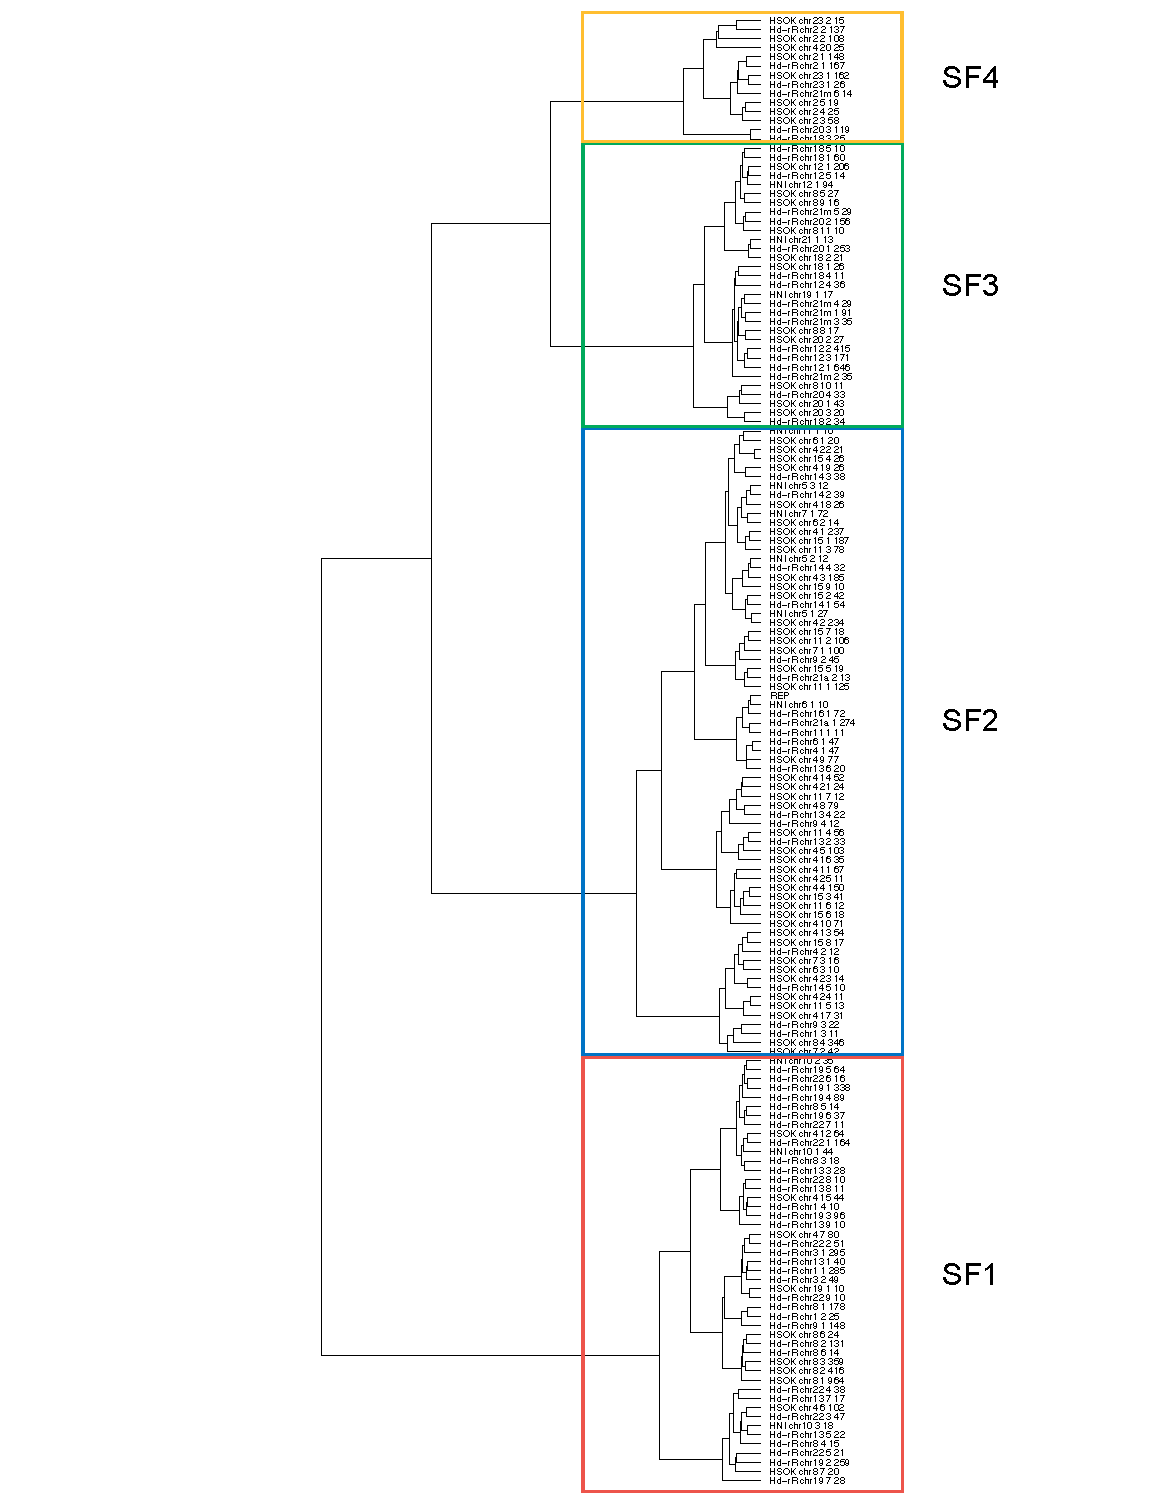
\includegraphics[width=\linewidth]{monomers_clustering.pdf}
    \caption{
      Hierarchical clustering of chromosome-representative monomers. Monomers are labeled as species, chromosome, cluster index, number of the cluster constituents. The clustering revealed four large subfamilies of satellite monomers.
    }
    \label{monomer_clustering}
  \end{figure*}

  \begin{table*}
    \centering
    \caption{Super-chromosomal subfamilies of centromeric repeats}
    \begin{tabular}{p{0.6cm}p{3.4cm}p{1.5cm}p{2cm}p{4.5cm}p{3.7cm}}
  \hline
  SF & Hd-rR & HNI & HSOK & combined & positions \\ \hline
  1 & 4,6,9,11,14,16,21a (1,13) & 5,6,7,11    & 4,6,7,11,15 (8) & 4,5,6,7,9,11,14,15,16,21a (1,8,13) & 1M+1SM+14A (2SM+1A) \\
  2 & 1,3,8,9,13,19,22          & 10          & 8,19 (4)        & 1,3,8,9,10,13,19,22 (4)            & 6SM+2ST+2A (1M) \\
  3 & 12,18,20,21m (8)          & 12,21 (19)  & 12,18,20 (8)    & 12,18,20,21m (8,19)                & 1M+8SM+2ST+1A (2SM) \\
  4 & 2,23 (21m)                &             & 2,23 (4)        & 2,23 (4,21m)                       & 3M+1SM (2M) \\
  \hline
\end{tabular}

    \label{super_chromosomal_subfamily}
    \caption*{{\small
      Chromosomes were classified into four subfamilies (SF). Chromosomes in brackets are the ones that have significantly more amount of repeats classified into another subfamily. Hd-rR chromosome 21 possessed two distantly-positioned arrays, thus is notated as 21m (metacentric) and 21a (acrocentric; see Table \ref{centromeric_repeat_distribution} for detail). Summarizing the chromosomes from the three strains, 22 out of the 24 chromosomes were assigned to one or two subfamilies. Notation of the centromeric positions are the same as Table \ref{centromeric_repeat_distribution}.
    }}
  \end{table*}


\subsection*{Sequence organization at the centromeres}
  Sequence organization on the assembled centromeric sequences were analyzed. Dot plot of centromeric sequences of each chromosome are shown in Supplementary Figure \ref{centromere_landscape}.

  HSOK chromosome 8 captured the longest centromeric arrays, namely two arrays of 250\,kb and 95\,kb flanking an assembly gap (Fig.\,\ref{chr8_browser}A). These two arrays comprised of the satellites from three subfamilies (SF\,1, SF\,2, SF\,3). SF\,1 satellites comprise large inner portion of the arrays, interspersed by SF\,2 satellites; these sequences were flanked by much less amount of SF\,3 satellites. Multiple alignment of the chromosome-representative monomers revealed that the representative monomer of the forth largest cluster which belongs to SF\,2 possessed $\sim$10-bp insertion compared to the representative monomers belonging to SF\,1, yet otherwise looks virtually identical (Fig.\,\ref{chr8_multiple_alignment}). The assignment of these representative monomers to the different subfamilies was due to the definition of the distance used for the hierarchical clustering, which was calculated by alignment identity of two sequences and thus large indels lead to substantial loss in the identity. On the other hand, the representative monomers belonging to SF\,3 exhibit distinct sequence composition from the monomers in SF\,1 and SF\,2. Interestingly, the orientation of the satellite sequences switched at the boundaries of SF\,1 and SF\,3 arrays (Fig.\,\ref{chr8_browser}A). This suggests the scenario that the SF\,1 array inserted into the SF\,3 array as a result of a sequence conversion, unequal crossover or other chromosome rearrangement events. Switches of sequence orientation in satellite arrays have also been observed in the pericentromeric regions of human chromosomes \cite{M.KatharineRuddand2004}. Overall similar sequence organization was observed in the same chromosome of Hd-rR, which had 20-kb and 40-kb SF\,1 arrays flanking an assembly gap and a 1-kb SF\,3 array at outside of the 20-kb SF\,1 array (Fig.\,\ref{chr8_browser}B).

  Another interesting example was HSOK chromosome 4 which captured a over 300-kb nearly continuous array (Fig.\,\ref{chr4_browser}). This array comprised mainly of SF\,2 satellites, interspersed with shorter SF\,1 satellite arrays. Also small amount of SF\,4 satellites were observed in downstream portion. Furthermore, frequent switches of sequence orientation were observed, some of which correspond to the SF boundaries whereas others do not.

  Chromosome 12 was the only chromosome that all the three strain genomes captured $>$10-kb centromeric arrays. The Hd-rR assembly reached the centromeric region from the both sides; HNI reached from the p-arm side; HSOK reached from the q-arm side (Fig.\,\ref{chr12_transition}A). All the arrays comprised of SF\,3 satellites. In order to examine if the sequences of these centromeric transitional regions are conserved among the strains, dot plots were drawn (Fig.\,\ref{chr12_transition}B,\,C). Whereas modest sequence conservation was observed in the surrounding unique regions, the sequence structure in the centromeric arrays were not conserved. Similar unconservation of sequence structures in centromeric transitional regions were observed in some other chromosomes (Fig.\,\ref{other_chroms_transition}). These results suggest that the repetitive sequences at the centromeres have evolved independently of surrounding unique regions, in line with traditional observations \cite{Willard1991}.

  % In addition to these outstanding examples, many other chromosomes had satellites of two or more SFs. In some of those chromosomes, similarly to the examples above, the different SF arrays positioned alternately or adjacently. In other chromosomes the different SF arrays located distantly, namely flanked by a contig gap or at the middle and an end of the same chromosome \ref{}.


  \begin{figure*}
    \centering
    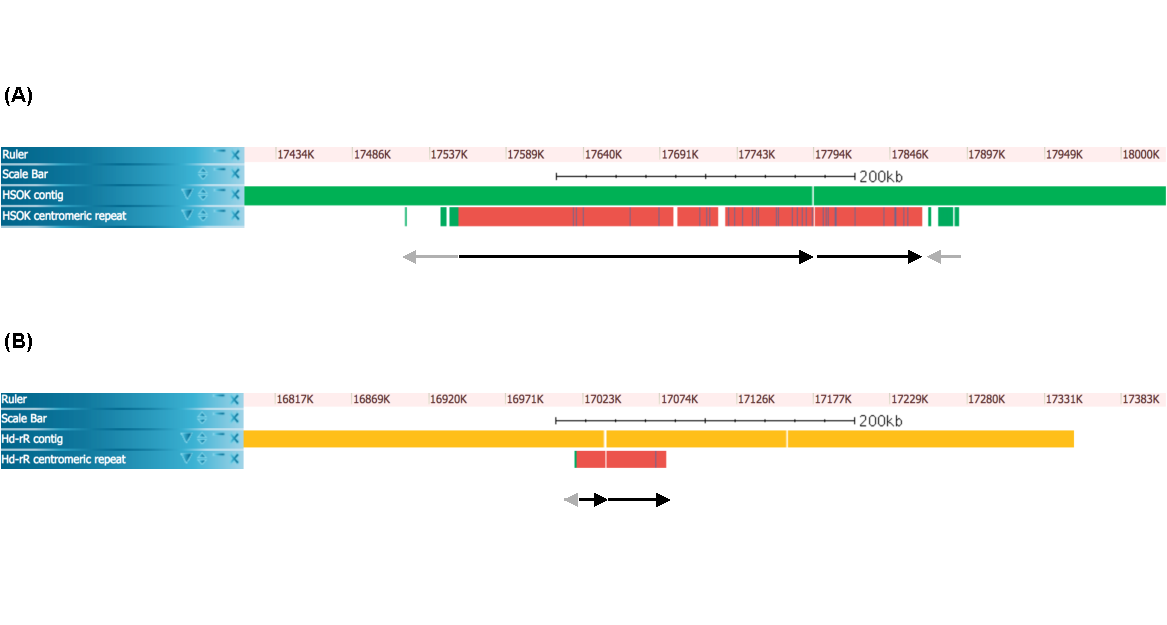
\includegraphics[width=\linewidth]{chr8_browser.pdf}
    \caption{
      Sequence organization of chromosome 8 centromeric regions. (A) HSOK chromosome 8 had 250-kb and 95-kb repeat arrays flanking an assembly gap. SF\,1 satellites (red) comprise large inner portion of the arrays, interspersed by SF\,2 satellites (blue). These sequences were flanked by shorter SF\,3 satellite arrays (green). The orientation of the satellite sequences switched at the boundaries of SF\,1 and SF\,3 arrays (indicated by black and grey arrows). (B) Hd-rR had similar sequence organization as HSOK.
    }
    \label{chr8_browser}
  \end{figure*}

  \begin{figure*}
    \centering
    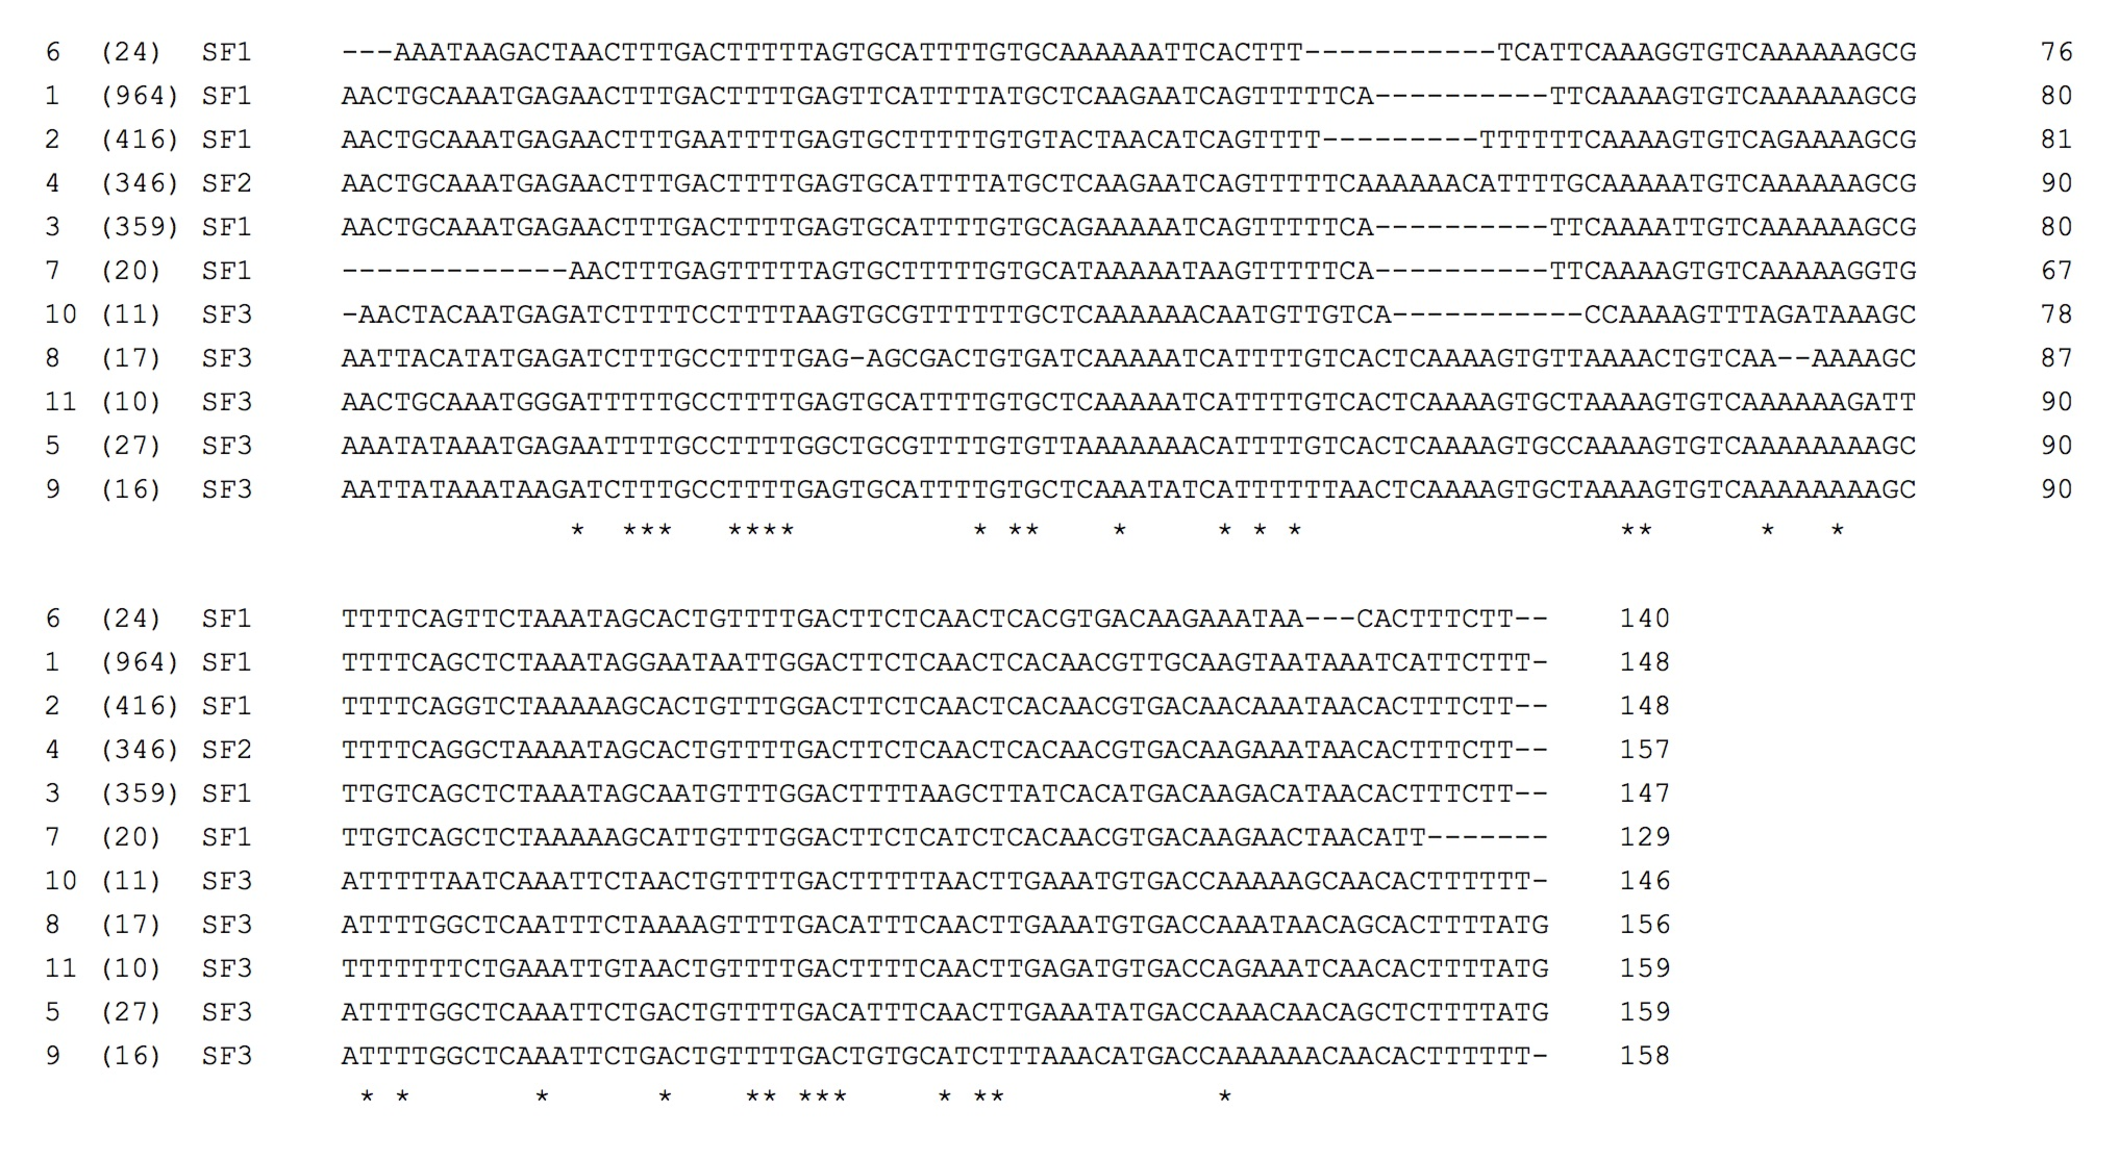
\includegraphics[width=\linewidth]{chr8_multiple_alignment.pdf}
    \caption{
      Multiple sequence alignment of HSOK chromosome 8 representative monomers. 11 representative monomers of HSOK chromosome 8 were aligned using Clustal Omega (version 1.2.3) \cite{Sievers2011}. The labels of each sequence represent cluster index (as a descending order of cluster size), number of monomers belonging to the cluster (in brackets) and belonging subfamilies. Asterisks ("*") indicate the nucleotides shared in all the representative monomers. Representative monomer 4 which belongs to SF\,2 has $\sim$10-bp insertion compared to SF\,1 representative monomers, yet otherwise shares virtually the same sequence composition. SF\,3 representative monomers have distinct sequence composition from SF\1, and SF\2 representative monomers.
    }
    \label{chr8_multiple_alignment}
  \end{figure*}

  \begin{figure*}
    \centering
    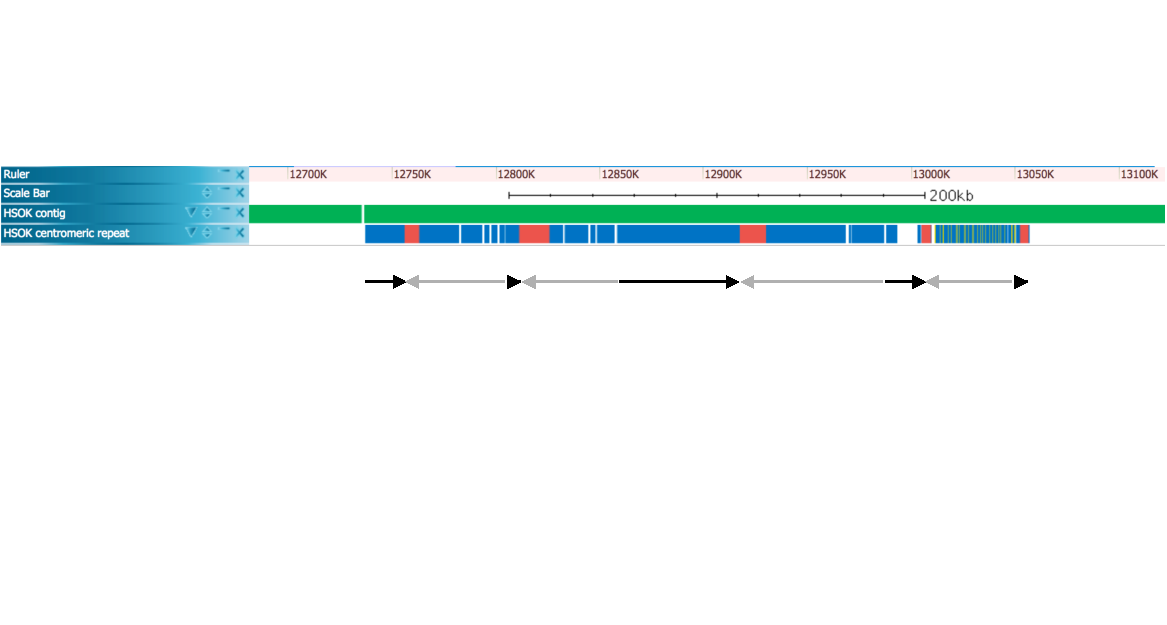
\includegraphics[width=\linewidth]{chr4_browser.pdf}
    \caption{
      Sequence organization of HSOK chromosome 4 centromeric region. The $\sim$300-kb nearly continuous array was truncated by the contig end at the left end. The array comprised mainly of SF\,2 satellites (blue) and these are interspersed by shorter SF\,1 satellite arrays (red). Also small amount of SF\,4 satellites (yellow) were observed in the right portion. Frequent switches of sequence orientation were observed (indicated by black and grey arrows).
    }
    \label{chr4_browser}
  \end{figure*}

  \begin{figure*}
    \centering
    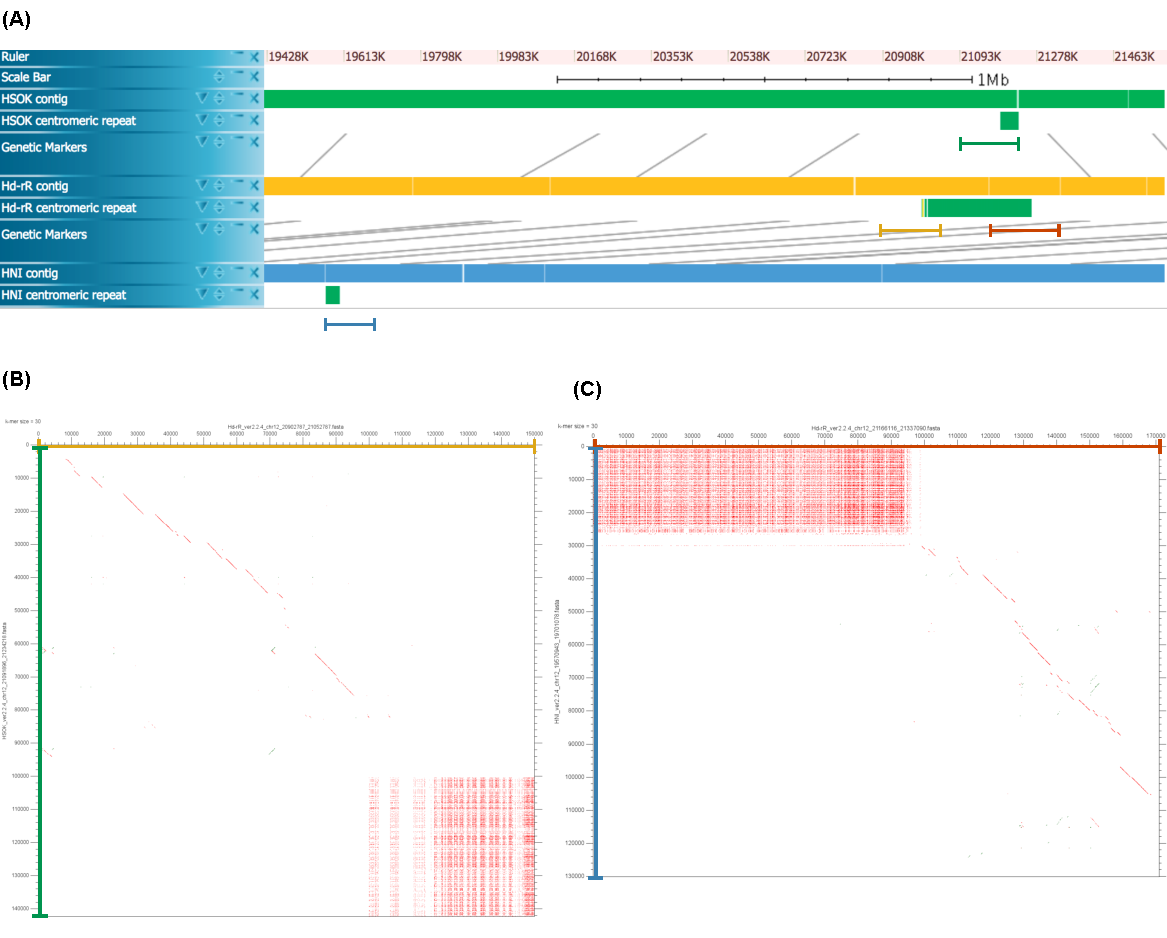
\includegraphics[width=\linewidth]{chr12_transition.pdf}
    \caption{
      Comparison of the centromeric transitional regions of chromosome 12. (A) The Hd-rR assembly reached the centromeric region from the both sides (separated by a contig gap); HNI reached from the p-arm side; HSOK reached from the q-arm side. The grey lines indicate the positions of corresponding genetic markers. (B) Sequences of the q-arm transitional regions of Hd-rR and HSOK was compared. (C) Sequences of the p-arm transitional regions of Hd-rR and HNI was compared. Dots represent 30-bp exact matches between two sequences. Whereas modest conservation was observed in the surrounding unique sequences (indicated by the chained diagonal lines), no clear conservation was observed within the centromeric array sequences.
    }
    \label{chr12_transition}
  \end{figure*}

% \subsection*{HOR structures}
%   Dot plot of the centromeric sequences revealed the presence of higher-order repeats (HORs) in many chromosomes.
